\documentclass{scrartcl}
\usepackage[utf8]{inputenc}
\usepackage[nonumberlist]{glossaries}
\usepackage{verbatim}
\usepackage{enumitem}
\usepackage{graphicx}
\title{Android Go App - Pflichtenheft}

\begin{document}
	\maketitle
	\newpage
	
	\tableofcontents
	\newpage
	
	\section{Zielbestimmung}
	\subsection{Musskriterien}
		\begin{itemize}
		\item Anmeldung mit Googleservices
		\item Ein User kann Mitglied mehrerer Gruppen sein und kann über diese Informationen abrufen.
		\item Gruppenverwaltung
			\begin{itemize}
			\item Erstellen neuer Gruppen.
			\item Suche bestehender Gruppen.
			\item Gründer, User Rollenstruktur.
			\item Mitglieder in die Gruppe aufnehmen, aus der Gruppe entfernen.
			\end{itemize}
		\item Terminverwaltung
			\begin{itemize}
			\item Termine können mit Zeit, Ort, Name innerhalb einer Gruppe erstellt werden.
			\item User können bei Terminen zu-/absagen.
			\item User werden an ihren Termin erinnert.
			\end{itemize}
		\item Ein User kann seinen eigenen Standort und den Gruppenmittelpunkt abrufen.	
		\end{itemize}
	\subsection{Wunschkriterien}
		\begin{itemize}
		\item "Bin Los" und "Bin da"
			\begin{itemize}
			\item User können per Button signalisieren ob sie bereits zum Treffpunkt unterwegs sind oder diesen sogar schon erreicht haben.
			\item Nur User die Unterwegs sind werden für den Gruppenmittelpunkt beachtet.
			\item User die den Treffpunkt erreicht haben werden für die Berechnung der Gruppenmitte stärker fokussiert.
			\end{itemize}
		\item Erinnerung an Termin auch bei geschlossener App.
		\item Termine können gelöscht und geändert werden
		\item Statistiken über Teilnahme der User speichern.
		\item QR-Code zum finden von Gruppen
		\item Sprachwahl
		\end{itemize}
	\subsection{Abgrenzungskriterien}
		\begin{itemize}
		\item Kein Chat.
		\item User können nicht die Standorte andere User abfragen.
		\end{itemize}

	\newpage

	

	\section{Produkteinsatz}
	\begin{itemize}	        
		\item Das Produkt soll das spontane Organisieren von Treffen unterstützen. Dazu soll es dem Nutzer möglich sein in einer Gruppe einen Termin zu erstellen, bzw. bei Terminen zu- und abzusagen.
		\item Kurz vor dem Termin wird dann der mittlere Standort der Gruppe angezeigt, um das Finden der anderen Gruppenmitglieder zu erleichtern.
		\end{itemize}
	\subsection{Andwendungsbereich}
		\begin{itemize}	        
		\item Spontane Terminvereinbarung 
		\end{itemize}
		\subsection{Zielgruppe}
		\begin{itemize}	        
		\item Alle Studierende und Mitarbeiter am KIT
		\end{itemize}
		\subsection{Betriebsbedingung}
		\begin{itemize}	        
		\item App kann überall eingesetzt werden
		\end{itemize}

	\newpage
	

	\section{Produktumgebung}
	\begin{itemize}	        
		\item Eine Client-Server Architektur
		\item Der Client ist eine Android-App
		\item Die App läuft parallel mit anderen Apps auf einem Android-Smartphone ohne mit diesen zu kommunizieren
		\end{itemize}
\subsection{Software}
		\begin{itemize}	        
		\item Client: Android ab 4.0
		\item Server: Tomcat 8
		\end{itemize}	
\subsection{Orgware}
		\begin{itemize}	        
		\item Internetverbindung und GPS
		\end{itemize}
		\subsection{Produktschnittstelle}
		\begin{itemize}	        
		\item Google Maps
		\end{itemize}
	\newpage


	\section{Funktionale Anforderungen}
		

		\subsection{Accountverwaltung}
		\begin{itemize}
		\item[FA10] Anmeldung eines Benutzers in der App über Googleservices.
		\item[FA20] Ersterfassung und Änderung des Benutzernamens.
		\end{itemize}
		
		\subsection{Gruppenverwaltung}
		\begin{itemize}
		\item[FA30] Jeder Benutzer kann eine Gruppe erstellen.
		\item[FA35] Ersterfassung und spätere Änderung des Gruppennamens durch den Gruppengründer.
		\item[FA40] Gruppen können über den Gruppennamen gesucht werden.
		\item[FA45] Benutzer können Beitrittsanfragen an eine Gruppen senden.
		\item[FA50]Der Gruppengründer kann Betrittsanfragen zu der Gruppe verwalten:
			\begin{itemize}
			\item Anfragen bestätigen, wodurch der Anfragende Mitglied der Gruppe wird und die Anfrage gelöscht wird.
			\end{itemize}
			\begin{itemize}
			\item Anfragen ablehnen, wodurch die Anfrage gelöscht wird.
			\end{itemize}
			\begin{itemize}
			\item Anfragen ignorieren, wodurch die Anfrage bestehen und sichtbar bleibt.
			\end{itemize}
		 \item[FA60] Der Gruppengründer kann bestehende Mitglieger aus der Gruppe entfernen.
		 \item[FA70] Die Gruppe kann durch den Gruppengründer gelöscht werden.
		 \item[FA80] Mitglieder der Gruppen, ausgenommen des Gruppengründers, können die Gruppe verlassen.
		 \item[FA90W] Der Gruppengründer kann seinen Status als Gruppengründer an ein Mitglied übergeben.
		\end{itemize}
		
		\subsection{Terminverwaltung}
		\begin{itemize}
		\item[FA100] Jedes Mitglied einer Gruppe kann einen Termin erstellen.
		\item[FA110] Der Terminersteller kann den von ihm erstellten Termin verwalten:
			\begin{itemize}
			\item Ersterfassung und Änderung des Terminzeitpunktes.
			\end{itemize}
			\begin{itemize}
			\item Ersterfassung und Änderung des Terminortes.
			\end{itemize}
			\begin{itemize}
			\item Ersterfassung und Änderung des Terminnamens.
			\end{itemize}
			
		\item[FA120] Der Termin wird jedem Gruppenmitglied angezeigt.
		\item[FA130] Jedes Gruppenmitglied kann einem Termin zu- oder absagen.
		\item[FA140] Jeder Teilnehmer wird vor Beginn des Termins benachrichtigt werden.
		
		\end{itemize}
		
		
		
		
	\newpage


	\section{Produktdaten}

	\newpage


	\section{Qualitäts-Anforderungen}
	\begin{itemize}[nosep] 
	\item[QA10] Die App soll auf jede Anfrage innerhalb von 5 Sekunden reagieren.
	\item[QA20] Die App fährt innerhalb von 10 Sekunden hoch.
	\item[QA30] Jede Funktion der App ist mit höchstens 5 Eingaben vom Startbildschirm zu erreichen.
	\item[QA40] Die Server sind immer über die App zu erreichen.
	\item[QA50] Die App fällt nicht aus, auch bei widrigen Bedingungen (kein Netzwerkverbinndung, Standortungenauigkeit).
	\item[QA60] Unterstützt bis zu 20 User pro Gruppe.
	\item[QA70] Jeder User kann in bis zu 10 Gruppen Mitglied sein.
	\item[QA80] Übersichtliche UI
	\end{itemize}

	\newpage


	\section{Globale Testfälle}

	\newpage


	\section{Systemmodelle}
	
	\subsection{Anwendungsfalldiagramm}
	\begin{figure}[h]
	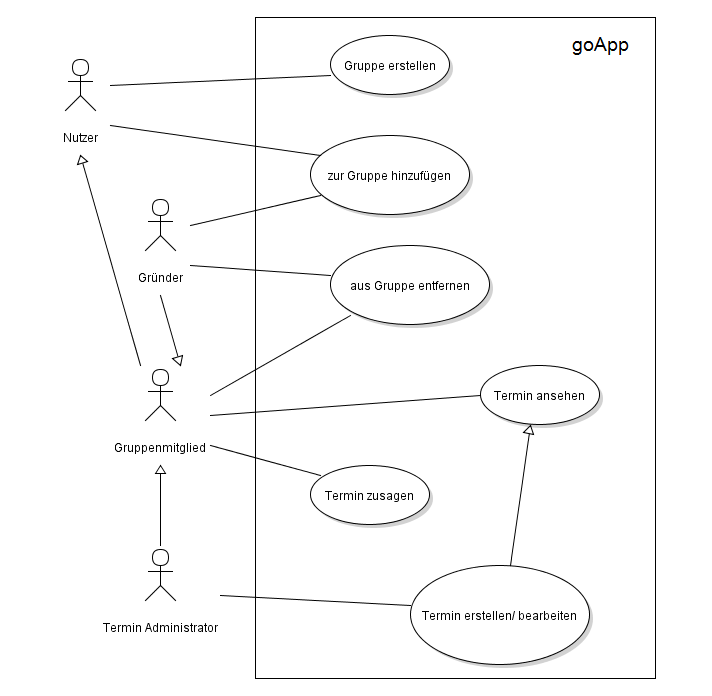
\includegraphics[width=\textwidth]{goApp_useCase}
	\end{figure}

	\newpage
	
	\begin{comment}
	\makeglossary


	\newglossaryentry{Gruppengründer} 
	{
	name=Gruppengründer,
	description={Bezeichnet den Status des Mitglieds, das die Gruppe gegründet hat. }
	}
	
	\newglossaryentry{Mitglied}
	{
	name=Miglied,
	description={Benutzer der einer Gruppe angehört.}
	}
	
	\newglossaryentry{Teilnehmer}
	{
	name=Teilnehmer,
	description={Ein Mitglied, das an einem Termin teilnimmt}
	}
	\end{comment}
	
	
\end{document}
